\subsection{Shorter does not imply faster}

\begin{figure}[h]
  \footnotesize
  \centering
  \begin{tikzpicture}[
    % type of arrow head
    &gt;=stealth',
    % keep arrow head from touching the surface
    shorten &gt;= 1pt,
    % automatic node positioning
    auto,
    % 
    node distance=2cm,
    % line thickness
    thick,
    bend angle=10,
    graybox/.style = {draw=gray!20, fill=gray!20, rounded corners},
    line/.style = {-&gt;, draw=black, thick},
    box/.style = {circle, draw=blue!50, fill=blue!20, minimum size=4mm}
    ]
 
    \coordinate (S) at (-5cm, 0.5cm);
    \coordinate (S1) at (-1.5cm, 1.5cm);
    \coordinate (S2) at (-1.5cm, -0.5cm);
    \coordinate (T) at (2cm, 0.5cm);
 
     % nodes
    \node (Sbox)  [box] at (S)  {s};
    \node (Sbox1) [box] at (S1) {$1$};
    \node (Sbox2) [box] at (S2) {$2$};
    \node (Tbox) [box] at (T) {t};
 
    % edges
    \path[line] (Sbox) -- node [above] {1} (Sbox1);
    \path[line] (Sbox) -- node [below] {1} (Sbox2);
	\path[line] (Sbox1) -- node [above] {1} (Tbox);
	\path[line] (Sbox2) -- node [below] {1} (Tbox);
	    
   \end{tikzpicture}
 \end{figure}
\todo[inline]{tilføj enheder}


\begin{figure}
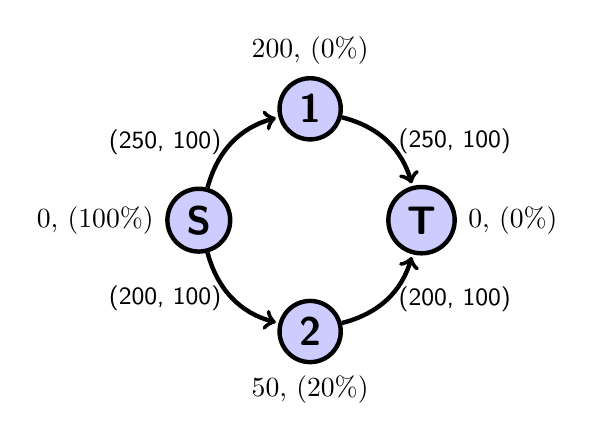
\begin{tikzpicture}[
->,
->,
shorten >=1pt,
auto,
node distance=2cm,
ultra thick,
main node/.style={circle,
								fill=blue!20,
								draw,
								font=\sffamily\Large\bfseries}]
%1
  \node[main node] (1) {1};
  \node[above] at (1.north) {200, (0\%)};
%2 
 \node[main node] (2) [below left of=1] {S};
  \node[left] at (2.west) {0, (100\%)};
%3 
 \node[main node] (3) [below right of=2] {2};
  \node[below] at (3.south) {50, (20\%)};
%4 
 \node[main node] (4) [below right of=1] {T};
  \node[right] at (4.east) {0, (0\%)};
%paths
  \path[every node/.style={font=\sffamily\small}]
    (1)
      edge [bend left] node[right] {(250, 100)} (4)
    (2) edge [bend right] node[left] {(200, 100)} (3)
          edge [bend left] node[left] {(250, 100)} (1)
    (3) edge [bend right] node[right] {(200, 100)} (4)
    (4) ;
\end{tikzpicture}
\label{fig:simpleroad-network}
\caption{A simple road-network with starting point s and end point t. Charge rate dictates that the longer path is the fastest}
\end{figure}

\begin{figure}
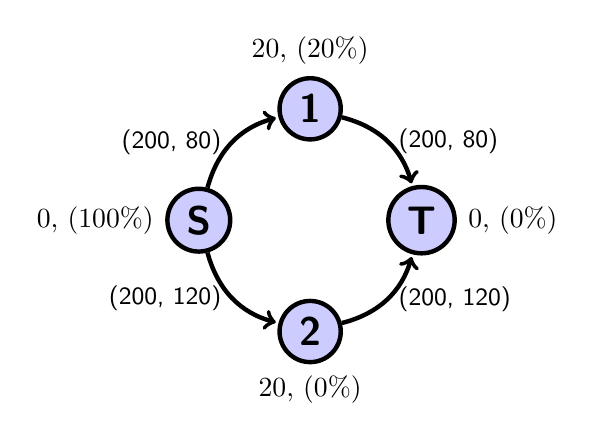
\begin{tikzpicture}[->,->,shorten >=1pt,auto,node distance=2cm,
 ultra thick,main node/.style={circle,fill=blue!20,draw,font=\sffamily\Large\bfseries}]
%1
  \node[main node] (1) {1};
  \node[above] at (1.north) {20, (20\%)};
%2 
 \node[main node] (2) [below left of=1] {S};
  \node[left] at (2.west) {0, (100\%)};
%3 
 \node[main node] (3) [below right of=2] {2};
  \node[below] at (3.south) {20, (0\%)};
%4 
 \node[main node] (4) [below right of=1] {T};
  \node[right] at (4.east) {0, (0\%)};
%paths
  \path[every node/.style={font=\sffamily\small}]
    (1)
      edge [bend left] node[right] {(200, 80)} (4)
    (2) edge [bend right] node[left] {(200, 120)} (3)
          edge [bend left] node[left] {(200, 80)} (1)
    (3) edge [bend right] node[right] {(200, 120)} (4)
    (4) ;
\end{tikzpicture}
\label{fig:simpleroad-network}
\caption{A simple road-network with starting point s and end point t. Consumption rate dictates that the longer path is the fastest}
\end{figure}

A shorter path does not necessarily imply a faster path for electrical vehicles. This is partly due to the fact that electrical vehicles use polynomially more energy as its speed increases but also due to the fact that charge times on charge stations varies a lot. 
Driving a longer path with a fast charge station on, can therefore turn out to be a faster choice than driving a shorter path with a slow charge station on. This is illustrated in Figure \ref{fig:simpleroad-network}. In the example, we assume our car has a battery capacity of 100 kWh and a consumption rate of 0,4 kWh/km at the speed of 100 km/h. Path 1 consist of two edges with distance = 250 km and speed limit = 100 km/t
and a charge station with a charge speed of 200 kW. Path 2 consist of two edges with
distance 200 km and speed limit 100 km/t and a charge station with a charge speed of 30 kW. The current battery capacity of the vehicle is noted at each vertex in parenthesis. The total time of each path:
				
\textbf{Path 1:} \text{route time} = ((250km + 250km) / 100km/h) + (100kWh / 200kW) = 5,5h
				
\textbf{Path 2:} \text{route time} = ((200 km + 200 km) / 100 km/h) + (60 kWh / 30 kW) = 6 h

\todo[inline]{mention other factors which dictates the fastest path}
